\section{Messwerte und Auswertung} % (fold)
\label{sec:messwerte_und_auswertung}

	\subsection{Michelson-Interferometrie} % (fold)
	\label{sub:michelson_interferometrie}
	
		\subsubsection{Fizeau-Streifen und Haidinger Ringe} % (fold)
		\label{ssub:fizeau_streifen}

			Die Interferenzen gleicher Dicke wurden durch Verkippen von Spiegel 2 erzeugt.
			Dabei entstanden die horizontalen Streifen aus Abbildung \ref{fig:fizeau-h-1} durch Drehung um die horizontale $y$-Achse senkrecht zur Verschiebungsrichtung $x$.
			Analog ließen sich die vertikalen Interferenzmuster durch Drehung um die Vertikale, also die z-Achse bilden.
			Während man bei den senkrechten Interferenzmuster von Abbildung \ref{fig:fizeau-v} gerade Steifen erkennt, die zur Seite jedoch einen größeren Abstand aufweisen, sieht man die Streifen von Abbildung \ref{fig:fizeau-h-1} in annähernd gleichem Abstand, jedoch verzerrt.
			Beides spricht in diesem Fall für eine Spiegelkrümmung einer der beiden Spiegel in $z$-Richtung.
		
			\begin{figure}[htb]
				\begin{subfigure}[b]{.45\textwidth}
					\centering
					\includegraphics[scale=0.07]{messwerte/fizeau-streifen-h-1.png}
					\caption{Drehung um $y$-Achse}
					\label{fig:fizeau-h-1}
				\end{subfigure}
				\begin{subfigure}[b]{.55\textwidth}
					\centering
					\includegraphics[scale=0.0775]{messwerte/fizeau-streifen-v-1.png}
					\caption{Drehung um $z$-Achse}
					\label{fig:fizeau-v}
				\end{subfigure}
				\caption{Fizeau-Streifen durch Interferenz der grünen Hg-Dampflinie bei $\lambda = 546 \unit{nm}$}
			\end{figure}

			Mit Hilfe des Maxima-Abstandes und der unter \ref{sub:interferenzen_gleicher_dicke_fizeau_streifen} angegebenen Formel, kann man in etwa den Winkel der Verkippung ausrechnen.
			Um die Abstände zu normieren wird angenommen, dass das Bild nur durch die letzte Linse vergrößert wird und somit der ursprüngliche Durchmesser des Bildes gleich dem Linsendurchmesser ist, welcher im Versuch zu $D = 3 \unit{cm} $ bestimmt wurde.
			Im Durchschnitt beträgt der Streifenabstand der senkrechten Streifen dann in etwa $a = 0.75 \unit{cm}$.
			\[ \implies \quad \sin(\alpha /2) = \frac{\lambda}{2 a} = \frac{546 \unit{nm}}{2 \cdot 0.75 \unit{cm}} 
			\approx 3.64 \cdot 10^{-5} \]
			\[ \implies \quad \alpha \approx 7.3 \cdot 10^{-5} = 15\,^{\prime\prime} \]
			Betrachtet man den zweit untersten horizontalen Streifen in Abbildung \ref{fig:fizeau-h-1} dann beträgt die Höhendifferenz zwischen Mitte und Rand in etwa die gesamte Breite des Maximums.
			Folglich wird die Abweichung von der planen Fläche eines der beiden Spiegel auch in dem Bereich von $\lambda$ also etwa $0.5\,\mu\mathrm{m}$ liegen.

			Die Haidinger-Ringe konnten mit etwas Feingefühl zwar eingestellt werden und zeigten auch das unter \ref{sub:interferenzen_gleicher_neigung_haidinger_ringe} gezeigte Verhalten, ließen sich allerdings aufgrund des schwachen Kontrastes und der geringen Leuchtstärke im Vergleich zu anderen Reflexen nicht durch die Kamera aufnehmen.


		% subsubsection fizeau_streifen (end)

		\subsubsection{Einlfuss der Glasplatte} % (fold)
		\label{ssub:einlfuss_der_glasplatte}

			Das MIF findet auch Anwendung bei der Bewertung der Güte optischer Bauteile.
			Als Beispiel wurde hier der Einfluss einer scheinbar planparallelen Glasplatte auf die Interferenzmuster untersucht.
			Dazu stellten wir zunächst eine möglichst geringe Spiegelverschiebung ein, also den Bereich der Haidinger-Ringe, zu erahnen in Abbildung \ref{fig:ohne_platte}.
			Als nächstes wurde die Platte in Strahlengang 2 gestellt.
			Wie man in Bild \ref{fig:mit_platte} sehen kann tauchen nun Fizeau-Streifen auf, was bedeutet, dass die Platte einen ähnlichen Einfluss wie die Spiegelverkippung hat.
			Daraus folgt, dass sie an einer Seite dicker sein muss als an der anderen und dadurch der optische Weg hier verlängert wird.
			In Aufnahme \ref{fig:mit_platte} ist zu erkennen, dass der Unterschied auf den Diagonalen am größten sein muss.
			Das Erscheinen von 5 Streifen bedeutet eine maximale Wegdifferenz von $5 \lambda$.
			Für die Glasplatte mit einem Brechnungsindex von $n_\m{Glas}=1.5$ bedeutet das eine Stärkendifferenz von:
			\[ \Delta d = \frac{5 \lambda}{2 (n_\m{Glas} - n_\m{Luft}) } \approx 2.7\,\mu\m{m} \]

			\begin{figure}[htb]
				\begin{subfigure}[b]{.5\textwidth}
					\centering
					\includegraphics[scale=0.07]{messwerte/harded-fucked-in-budapest-1.png}
					\caption{Ohne Glasplatte}
					\label{fig:ohne_platte}
				\end{subfigure}
				\begin{subfigure}[b]{.5\textwidth}
					\centering
					\includegraphics[scale=0.069]{messwerte/harded-fucked-in-budapest-2-extended-unedited-directors-cut.png}
					\caption{Mit Glasplatte}
					\label{fig:mit_platte}
				\end{subfigure}
				\caption{Interferenzmuster am MIF bei minimaler Wegdifferenz bei verwendeter Wellenlänge $\lambda = 546\unit{nm}$}
			\end{figure}
		
		% subsubsection einlfuss_der_glasplatte (end)

		\subsubsection{Weißlichtinterferenz} % (fold)
		\label{ssub:wei_lichtinterferenz}

			Auch das Licht eines thermischen Strahlers kann am MIF zur Interferenz gebracht werden.
			In Abbildung \ref{fig:weiss} ist dies zu sehen.
			Die Anforderung hierbei ist den sehr kleinen Bereich der Kohärenzlänge $l_\m{koh}$ genau einzustellen.
			Durch Verkippen von Spiegel 2 konnten wir nun wie im Bild zu erkennen maximal 7 Fizeau-Streifen erzeugen, bis die Wegdifferenz $2 \Delta x > l_\m{koh}$ war.
			Wenn wir für weißes Licht eine mittlere Wellenlänge von etwa $\overline{\lambda} = 550 \unit{nm} $ einsetzen erhalten wir als Abschätzung für die Kohärenzlänge:
			\[ l_\m{koh} = 7 \overline{\lambda} \approx 3.8\,\mu\m{m} \]

			\begin{figure}[htb]
				\centering
				\includegraphics[scale=0.13]{messwerte/weiss-1.png}
				\caption{Interferenz einer Weißlichtquelle (Glühlampe) am MIF}
				\label{fig:weiss}
			\end{figure}

		% subsubsection wei_lichtinterferenz (end)


		\subsubsection{Inhomogener Brechungsindex durch Wärme} % (fold)
		\label{ssub:inhomogener_brechungsindex_durch_w_rme}
			
			Die Empfindlichkeit des MIF konnte im Versuch mit einem heißen Widerstand demonstriert werden.
			Der Widerstand wurde im Strahlengang vor Spiegel 2 positioniert und die Luft über ihm erwärmt.
			Daraus resultierte eine Verminderung des Brechungsindex, was zu einer Verkürzung der optischen Weglänge führt.
			In Abbildung \ref{fig:hot ohm a} ist das Interferenzmuster mit eingebrachten Widerstand zu sehen.

			\begin{figure}[htb]
				\centering
				\includegraphics[scale=0.11]{messwerte/hot-ohm-a.png}
				\caption{Interferenzstreifen der grünen Hg-Dampflinie bei $\lambda = 546 \unit{nm}$ mit Wärmequelle im Strahlengang}
				\label{fig:hot ohm a}
			\end{figure}

			Man sieht, dass die regelmäßigen Fizeau-Streifen im linken Bereich verzerrt sind.
			Hier ist der Strahl durch heißere Luft propagiert.
			Die maximale Verschiebung kann anhand der Abbildung auf etwa ein $\lambda$ geschätzt werden.
			Damit ergibt sich über den insgesamt etwa $2 \unit{cm}$ langen Widerstand eine Weglängendifferenz von:
			\[ \lambda = 2\cdot 2 \unit{cm} \cdot (n_\m{cold} - n_\m{hot}) \]
			\[ \implies \quad \Delta n \approx 1.4\cdot 10^{-5} \]

		% subsubsection inhomogener_brechungsindex_durch_w_rme (end)

	% subsection michelson_interferometrie (end)

	\subsection{Fourier-Spektroskopie} % (fold)
	\label{sub:fourier_spektroskopie}

		\subsubsection{Parameter und Auflösevermögen} % (fold)
		\label{ssub:parameter_und_aufl_severm_gen}

			Zum Verdeutlichen des Prinzips, des Fourier-Spektrometers (FS) wurden zunächst zwei Schwingungen am Frequenzgenerator erzeugt und überlagert.
			Diese besaßen eine geringe Frequenzdifferenz $\Delta f$, um somit eine Schwebung zu erzeugen.
			Die FFT des Interferogramms ist in den Abbildungen \ref{fig:schwebung-1} und \ref{fig:schwebung-2} für verschiedene Aufnahmeparameter zu sehen.
			Es ist natürlich zu beachten, dass die unten angegebene Wellenlänge hier nicht der wirklichen Wellenlänge der Signale entspricht, was aber für das Auflösevermögen keine Rolle spielt.
			Wie man klar erkennen kann, können die beiden Frequenzen im ersten Bild aufgelöst werden, währenddessen sich im zweiten Bild aufgrund der geringen Sampleanzahl die Auflösung verschlechtert und somit die einzelnen Peaks nicht mehr getrennt werden können.
			Mit der Gleichung welche in Grundlagen unter Abschnitt \ref{sub:fourierspektroskopie} angegeben ist, lässt sich nun das Auflösungsvermögen für beide Aufnahmen berechnen.
			Zu beachten ist hier die Annahme, dass der Motor die konstante Geschwindigkeit $v = 10\,\mu\m{m}s^{-1}$ hält.
			Die jeweilige Aufnahmezeiten $T$ beträgt jeweils $S/sps$ und die Wellenlängen liegen im Bereich um $504 \unit{nm}$.
			\[ \curvb{\frac{\lambda}{\Delta \lambda}}_1 = \frac{2 v T_1}{\lambda} \approx 3900,\qquad \curvb{\frac{\lambda}{\Delta \lambda}}_2 = \frac{2 v T_2}{\lambda} \approx 39 \]
			Für das minimal benötigte Auflösungsvermögen gilt:
			\[ \curvb{\frac{\lambda}{\Delta \lambda}}_\m{min} = \frac{504 \unit{nm}}{2 \unit{nm}} \approx 250 \]

			\begin{figure}[htb]
				\centering
				\input{schwebung-1}
				\caption{FFT des Interferogramms der überlagerten Sinusschwingungen mit $1000\unit{sps}$ und $100000$ Samples}
				\label{fig:schwebung-1}
			\end{figure}

			\begin{figure}[htb]
				\centering
				\input{schwebung-2}
				\caption{FFT des Interferogramms der überlagerten Sinusschwingungen mit $500\unit{sps}$ und $500$ Samples}
				\label{fig:schwebung-2}
			\end{figure}
 
		% subsubsection parameter_und_aufl_severm_gen (end)

		\subsubsection{Spektrum LED- und Gaslaser} % (fold)
		\label{ssub:spektrum_led_und_gaslaser}

			Im Folgenden wurden einige einfache Vergleichsspektren verschiedener LED- und Laserlichtquellen vermessen.
			In Abbildung \ref{fig:gr-led-spec} sieht man die Intensitätsverteilung einer grünen Leuchtdiode.
			Wie erwartet und liegt das Maximum der Intensitätsverteilung im Bereich von $550 \unit{nm}$, was im Auge einen grünen Farbeindruck erweckt.
			Die relativ Breite Verteilung des Spektrums von ca. $520 bis 600 \unit{nm}$ ist mit der Bandstruktur des Halbleitermaterials zu erklären.
			Das Maximum der Intensität wurde zu ungefähr $540 \unit{nm}$ bestimmt.
			Damit gilt für die Bandlücke:
			\[ \Delta E = \frac{hc}{\lambda} \approx 2.3 \unit{eV} \]

			Dagegen ist Spektrum einer Laser-LED in Graph \ref{fig:rot-laser-led} gezeigt.
			Durch die Resonatoren und die hohe Intensität im Bauteil setzen sich hier nur 2 Moden durch, wobei die erste bei 34567890 nm wesentlich stärker ausgeprägt ist, als die zweite im Abstand von 978 nm.

			Im dritten Bild sieht man nun noch das Spektrum eines frequenzverdoppelten Nd:Yag-Lasers.
			Dieser erzeugt zunächst Licht der Wellenlänge $1064 \unit{nm}$ (Quelle Bergmann und Schäfer Seite 882) welches anschließend durch den nichtlinearen Prozess der Frequenzverdopplung in einem Kristall zu großen Teilen zu Licht der halben Wellenlänge, also $532 \unit{nm}$ umgewandelt wird.
			Da der Detektor nur bis etwa $1000 \unit{nm}$ empfindlich ist (siehe Abschnitt \ref{ssub:gl_hlampenspektrum}) kann die ursprüngliche Frequenz hier nicht mehr dargestellt werden.
			Dafür sieht man überdeutlich den Peak bei ziemlich genau $532 \unit{nm}$ wie erwartet.
			Da für die Frequenzverdopplung spezielle Anforderungen für Frequenz und Wellenlänge im Kristall gelten, können sich hier auch andere Moden, selbst wenn sie im Nd:YAG-Laser entstehen würden nicht mehr effektiv verdoppeln, weshalb selbst bei hoher Auflösung (hier etwa 8000) nur ein Peak zu sehen ist. 

		
			\begin{figure}[htb]
				\centering
				\input{led-spec}
				\caption{Spektrum einer grünen LED aufgenommen mit $10000$ Samples und $500 \unit{sps}$}
				\label{fig:gr-led-spec}
			\end{figure}

			\begin{figure}[htb]
				\centering
				\input{led-laser-spec}
				\caption{Spektrum einer roten Laser-LED aufgenommen mit $100000$ Samples und $1000 \unit{sps}$}
				\label{fig:rot-laser-led}
			\end{figure}

			\begin{figure}[htb]
				\centering
				\input{g-laser-spec}
				\caption{Spektrum eines grünen, frequenzverdoppelten Nd:YAG Lasers aufgenommen mit $100000$ Samples und $500 \unit{sps}$}
				\label{fig:nd-yaq-laser}
			\end{figure}

		% subsubsection spektrum_led_und_gaslaser (end)

		\subsubsection{Spektrum Natrium- und Quecksilberdampflampe} % (fold)
		\label{ssub:spektrum_natrium_und_quecksilberdampflampe}

			Um die Eignung des FS zur Untersuchung von Atomspektren zu überprüfen wurden die Intensitätsverteilungen von Natriumlampe und Quecksilberdampflampe aufgenommen und vermessen.
			Graph \ref{fig:na-spec} zeigt den charakteristischen Doppelpeak von Na bei ca. $589.0$ und $589.5 \unit{nm}$.
			Das der recht schmale Doppelpeak noch getrennt zu sehen ist, liegt wiederum am Auflösevermögen.
			Es beträgt im gezeigten Bild etwa:
			\[ \frac{200 \unit{s} \cdot 10 \,\mu\m{m}s^{-1}}{589 \unit{nm}} \approx 3400 \qquad > \qquad \frac{\lambda}{\Delta \lambda} = 1178 \]

			Das Quecksilberspektrum zeigt über einen sehr großen Bereich detailliert alle Peaks.
			Die ermittelten Wellenlängen stimmen auf den Nanometer mit dem Vergleichsspektrum aus Abschnitt \ref{sec:hg_spektrum} überein.
			\begin{table}[h]
				\begin{tabular}{r|rrrrr}
					Messwerte $[\unit{nm}]$ & $579.1$ & $576.9$ & $546.0$ & $435.8$ & $404.6$ \\
					\hline
					Tabellenwerte $[\unit{nm}]$ & $579$ & $577$ & $546.1$ & $435.8$ & $405$
				\end{tabular}
				\caption{Spektrallinien des Quecksilbers}
			\end{table}
			Allerdings erkennt man das im Bereich zwischen $436$ und $546 \unit{nm}$ etliche Spektrallinien fehlen, was mit ihrer zu geringen Intensität zu erklären ist.
			Auch hier genügt die Auflösung wieder für die zwei eng benachbarten Linien bei $577$ und $579 \unit{nm}$.


			\begin{figure}[htb]
				\centering
				\input{na-dd}
				\caption{Vergrößerter Ausschnitt aus dem Spektrum der Na-Lampe mit typischer Doppel-D-Linie,
				Aufnahme mit $200000$ Samples und $1000 \unit{sps}$}
				\label{fig:na-spec}
			\end{figure}

			\begin{figure}[htb]
				\centering
				\input{hg-spec}
				\caption{Breiter Bereich des Spektrums einer Hg-Dampflampe, 
				Aufnahme mit $100000$ Samples und $1000 \unit{sps}$}
				\label{fig:hg.spec}
			\end{figure}
			
		% subsubsection spektrum_natrium_und_quecksilberdampflampe (end)


		\subsubsection{Glühlampenspektrum und Detektorbandlücke} % (fold)
		\label{ssub:gl_hlampenspektrum}

			Speziell zur Analyse für Infrarotspektren wird häufig ein FS verwendet, da hier die Motoreinstellung leichter auf Wellenlängengenauigkeit einzustellen ist.
			Das Spektrum der Wolfram-Glühlampe ist in Abbildung \ref{fig:lamp-si} zu sehen.
			Hier wurde zur Aufnahme ein Si-Detektor mit einer Bandlücke von $1.12 \unit{eV}$ verwendet.\footnote{Quelle: Hunklinger Festkörperphysik S. 413}
			Offenbar reicht hier das Spektrum bis etwa $1070 \unit{nm}$ und hat sein Maximum im roten bei $900$.
			Die selbe Quelle mit einem PbSe-Detektor ausgewertet, wie in Abbildung \ref{fig:lamp-pbse} gezeigt, liefert ein ganz anderes Spektrum.
			Hier scheint das Spektrum bei $1000 \unit{nm}$ gerade erst anzufangen und hat sein Maximum bei $1650$ um dann weit im Infraroten bei ca. $2600 \unit{nm}$ abzuflachen.
			Die Ursache für den frühen Abbruch im Si-aufgenommenen Spektrum liegt an der relativ großen Bandlücke des Silizium Halbleiters.
			Mit Hilfe der Bandlückenenergie $E_\m{gap}$ kann die größtmögliche noch zu messende Wellenlänge bestimmt werden:
			\[ \lambda _ \m{max} = \frac{h c}{E_\m{gap}} \approx 1100 \unit{nm}\]
			Im Falle von PbSe mit $E_\m{gap} = 0.278 \unit{eV}$ ergibt sich analog\footnote{Quelle: \url{http://link.springer.com/chapter/10.1007/10681727_890#page-1}}
			\[ \lambda _ \m{max} \approx 4460 \unit{nm}\]
			Wie wir sehen liegt im Fall des Si-Detektors die Bandlückenenergie größer als die Energie der langwelligen Photonen, weshalb das Spektrum hier abbricht.
			Im Fall der PbSe-Detektors liegt $\lambda _ \m{max}$ weit außerhalb der Emission.
			Das Spektrum der Halogen-Lampe aus Abbildung \ref{fig:halo-pbse} zeigt einen ganz ähnlichen Verlauf mit Maximum in etwa an der gleichen Stelle.
			Die Halogen-Lampe wurde im weiteren Verlauf statt der Glühlampe verwendet weil sie sich besser eignete und sie nicht ansteuerbar war, weshalb sie stets die gleiche Leistung und das gleiche Spektrum hatte (und vor allem weil die Glühlampe durchgebrannt war).
			Beide Spektren (vom PbSe-Detektor) zeigen den typischen Verlauf eines schwarzen Strahlers.
			Es ist bemerkenswert, dass beide Lampen ihr eigentliches Maximum weit außerhalb des sichtbaren Lichtes haben, was die Vermutung über den schlechten Wirkungsgrad bestätigt.
			Der Knick bei ca. $1410 \unit{nm}$ entsteht durch das Absorptionsverhalten von Wasser und Kohlenstoffdioxid in der Atmosphäre, näheres dazu unter Abschnitt \ref{ssub:absorbtionsspektren_von_wasser_und_benzol}.


			\begin{figure}[htb]
				\centering
				% GNUPLOT: LaTeX picture with Postscript
\begingroup
  \makeatletter
  \providecommand\color[2][]{%
    \GenericError{(gnuplot) \space\space\space\@spaces}{%
      Package color not loaded in conjunction with
      terminal option `colourtext'%
    }{See the gnuplot documentation for explanation.%
    }{Either use 'blacktext' in gnuplot or load the package
      color.sty in LaTeX.}%
    \renewcommand\color[2][]{}%
  }%
  \providecommand\includegraphics[2][]{%
    \GenericError{(gnuplot) \space\space\space\@spaces}{%
      Package graphicx or graphics not loaded%
    }{See the gnuplot documentation for explanation.%
    }{The gnuplot epslatex terminal needs graphicx.sty or graphics.sty.}%
    \renewcommand\includegraphics[2][]{}%
  }%
  \providecommand\rotatebox[2]{#2}%
  \@ifundefined{ifGPcolor}{%
    \newif\ifGPcolor
    \GPcolorfalse
  }{}%
  \@ifundefined{ifGPblacktext}{%
    \newif\ifGPblacktext
    \GPblacktexttrue
  }{}%
  % define a \g@addto@macro without @ in the name:
  \let\gplgaddtomacro\g@addto@macro
  % define empty templates for all commands taking text:
  \gdef\gplbacktext{}%
  \gdef\gplfronttext{}%
  \makeatother
  \ifGPblacktext
    % no textcolor at all
    \def\colorrgb#1{}%
    \def\colorgray#1{}%
  \else
    % gray or color?
    \ifGPcolor
      \def\colorrgb#1{\color[rgb]{#1}}%
      \def\colorgray#1{\color[gray]{#1}}%
      \expandafter\def\csname LTw\endcsname{\color{white}}%
      \expandafter\def\csname LTb\endcsname{\color{black}}%
      \expandafter\def\csname LTa\endcsname{\color{black}}%
      \expandafter\def\csname LT0\endcsname{\color[rgb]{1,0,0}}%
      \expandafter\def\csname LT1\endcsname{\color[rgb]{0,1,0}}%
      \expandafter\def\csname LT2\endcsname{\color[rgb]{0,0,1}}%
      \expandafter\def\csname LT3\endcsname{\color[rgb]{1,0,1}}%
      \expandafter\def\csname LT4\endcsname{\color[rgb]{0,1,1}}%
      \expandafter\def\csname LT5\endcsname{\color[rgb]{1,1,0}}%
      \expandafter\def\csname LT6\endcsname{\color[rgb]{0,0,0}}%
      \expandafter\def\csname LT7\endcsname{\color[rgb]{1,0.3,0}}%
      \expandafter\def\csname LT8\endcsname{\color[rgb]{0.5,0.5,0.5}}%
    \else
      % gray
      \def\colorrgb#1{\color{black}}%
      \def\colorgray#1{\color[gray]{#1}}%
      \expandafter\def\csname LTw\endcsname{\color{white}}%
      \expandafter\def\csname LTb\endcsname{\color{black}}%
      \expandafter\def\csname LTa\endcsname{\color{black}}%
      \expandafter\def\csname LT0\endcsname{\color{black}}%
      \expandafter\def\csname LT1\endcsname{\color{black}}%
      \expandafter\def\csname LT2\endcsname{\color{black}}%
      \expandafter\def\csname LT3\endcsname{\color{black}}%
      \expandafter\def\csname LT4\endcsname{\color{black}}%
      \expandafter\def\csname LT5\endcsname{\color{black}}%
      \expandafter\def\csname LT6\endcsname{\color{black}}%
      \expandafter\def\csname LT7\endcsname{\color{black}}%
      \expandafter\def\csname LT8\endcsname{\color{black}}%
    \fi
  \fi
  \setlength{\unitlength}{0.0500bp}%
  \begin{picture}(6802.00,3968.00)%
    \gplgaddtomacro\gplbacktext{%
      \csname LTb\endcsname%
      \put(946,954){\makebox(0,0)[r]{\strut{} 0}}%
      \put(946,1454){\makebox(0,0)[r]{\strut{} 0.2}}%
      \put(946,1954){\makebox(0,0)[r]{\strut{} 0.4}}%
      \put(946,2453){\makebox(0,0)[r]{\strut{} 0.6}}%
      \put(946,2953){\makebox(0,0)[r]{\strut{} 0.8}}%
      \put(946,3453){\makebox(0,0)[r]{\strut{} 1}}%
      \put(1078,484){\makebox(0,0){\strut{} 400}}%
      \put(1744,484){\makebox(0,0){\strut{} 500}}%
      \put(2410,484){\makebox(0,0){\strut{} 600}}%
      \put(3076,484){\makebox(0,0){\strut{} 700}}%
      \put(3742,484){\makebox(0,0){\strut{} 800}}%
      \put(4407,484){\makebox(0,0){\strut{} 900}}%
      \put(5073,484){\makebox(0,0){\strut{} 1000}}%
      \put(5739,484){\makebox(0,0){\strut{} 1100}}%
      \put(6405,484){\makebox(0,0){\strut{} 1200}}%
      \put(176,2203){\rotatebox{-270}{\makebox(0,0){\strut{}Intensität}}}%
      \put(3741,154){\makebox(0,0){\strut{}Wellenlänge $\lambda \ [\unit{nm}]$}}%
    }%
    \gplgaddtomacro\gplfronttext{%
      \csname LTb\endcsname%
      \put(2398,3530){\makebox(0,0)[r]{\strut{}Messwerte}}%
    }%
    \gplbacktext
    \put(0,0){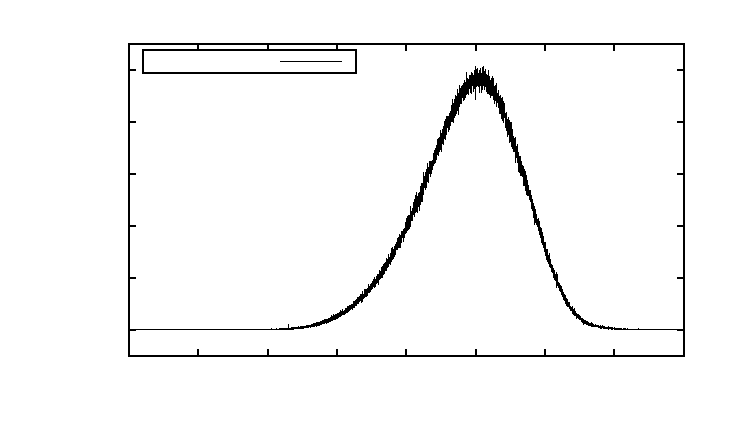
\includegraphics{lamp-spec}}%
    \gplfronttext
  \end{picture}%
\endgroup

				\caption{Spektrum einer herkömmlichen Wolfram-Glühbirne aufgezeichnet mit einem Siliziumdetektor 
				sowie $100000$ Samples und $500 \unit{sps}$}
				\label{fig:lamp-si}
			\end{figure}

			\begin{figure}[htb]
				\centering
				\input{lamp-pbse-spec}
				\caption{Spektrum einer herkömmlichen Wolfram-Glühbirne aufgezeichnet mit einem Bleiseleniddetektor 
				sowie $100000$ Samples und $500 \unit{sps}$}
				\label{fig:lamp-pbse}
			\end{figure}

			\begin{figure}[htb]
				\centering
				\input{halo-pbse-spec}
				\caption{Spektrum einer Halogenlampe aufgezeichnet mit einem Bleiseleniddetektor 
				sowie $10000$ Samples und $500 \unit{sps}$}
				\label{fig:halo-pbse}
			\end{figure}
		
		% subsubsection gl_hlampenspektrum (end)
	
		\subsubsection{Absorbtionsspektren von Wasser und Benzol} % (fold)
		\label{ssub:absorbtionsspektren_von_wasser_und_benzol}

			Um das Absorptionsverhalten der Substanzen zu Überprüfen wurde zunächst ein möglichst breitbandiges Referenzspektrum erstellt, dazu diente das Halogen-Spektrum aus Abbildung \ref{fig:halo-pbse}.
			Anschließend wurden kleine Proben der Flüssigkeiten in den Strahlengang zwischen Quelle und Kollimator gebracht.
			Das Ergebnis für Wasser ist in Graph \ref{fig:die Henne} gezeigt.
			Wie schon in Abbildung \ref{fig:halo-pbse} sehen wir die Absorption bei $1400 \unit{nm}$.
			Dies deckt sich mit der Referenz aus Anhang \ref{sec:absorptionsspektrum_wasser}.
			Allgemein lässt sich der Verlauf aus \ref{fig:die Henne} als Multiplikation der Spektren von Halogen-Lampe und Wasserdampfabsorption in der Atmosphäre begreifen.
			Für Benzol konnten leider keine verlässlichen Referenzen gefunden werden.
			Auch hier ist der Einbruch bei $1400 \unit{nm}$ zu sehen, der Peak bei ca. $600 \unit{nm}$ gestreutes Licht des Referenzlasers.

			\begin{figure}[htb]
				\centering
				\input{halo-h20-spec}
				\caption{Spektrum einer Halogenlampe nach Durchgang durch $2 \unit{cm}$ Wasser aufgezeichnet mit einem Bleiseleniddetektor 
				sowie $10000$ Samples und $500 \unit{sps}$}
				\label{fig:die Henne}
			\end{figure}
		
			\begin{figure}[htb]
				\centering
				\input{halo-benz-spec}
				\caption{Spektrum einer Halogenlampe nach Durchgang durch $2 \unit{cm}$ Benzol aufgezeichnet mit einem Bleiseleniddetektor 
				sowie $10000$ Samples und $500 \unit{sps}$}
				\label{fig:dich ins Knie}
			\end{figure}

		% subsubsection absorbtionsspektren_von_wasser_und_benzol (end)

	% subsection fourier_spektroskopie (end)

% section messwerte_und_auswertung (end)